\documentclass[10pt]{article}
\usepackage{amsmath}
\usepackage{amsfonts}
\usepackage{amssymb}
\usepackage{amsthm}
\usepackage{graphicx}   %Include graphics
\usepackage{float}      %Used to force graphics to stay where I want them to stay
\usepackage{mathrsfs}   %for Fourier transform 'F' symbol \mathscr{F}
\usepackage{hyperref}   %For hyperlinks in the PDF
\usepackage{enumitem}   %so we can have nonIndented lists and enumerations
\usepackage{caption}
\usepackage{subcaption}


\pdfpagewidth 8.5in
\pdfpageheight 11in
\setlength{\oddsidemargin}{-.35in}
\setlength{\textwidth}{7.32in}
\setlength{\topmargin}{-.6in}
\setlength{\textheight}{9.4in}

%%%%%%%%%%%%%%%%%%%%%%%%%%%%%%%%%%%%%%%%%%%%%%%%%%%%%%%%%%

%matrix macro
\newcommand{\mat}[2][ccccccccccccccc]{\left [\!\!\begin{array}{#1} #2\\ \end{array} \!\!\right]}
\newcommand{\determ}[2][ccccccccccccccc]{\left| \begin{array}{#1} #2\\ \end{array} \right| \vspace{.5em}}

%permutation
\newcommand{\perm}[2][ccccccccccccccc]{\left (\begin{array}{#1} #2\\ \end{array} \right) \vspace{.5em}}

%piecewise function
%  example:
%     $$H_i(K, K_0)\iso\piece{ \trivial & \text{if $i=0$} \\ \bbz/2\bbz &\text{if $i=1$} \\ \trivial & \text{if $i\ge2$}}$
%
\newcommand{\piece}[2][cll]{\left \{\begin{array}{#1} #2\\ \end{array} \right. }

%system of equations
\newcommand{\sys}[2][lll]{\left \{\begin{array}{#1}#2 \\ \end{array} \right. }

%integral
\newcommand{\dint}{\displaystyle\int}

%sum
\newcommand{\dsum}[3]{
           \displaystyle\sum_{#1}^{#2} #3 }

%sum start i=0
\newcommand{\dsumiz}[2]{
           \displaystyle\sum_{i=0}^{#1} #2}

%sum start i=1
\newcommand{\dsumio}[3]{
           \displaystyle\sum_{i=1}^{#2} #3 }


%sets {b,...,e} and sets with conditions {x | x is an integer}
\newcommand{\set}[2]{  \left\{#1,\ldots,#2\right\} }
\newcommand{\dset}[2]{  \left\{#1\; :\;\;#2\right\} }
\newcommand{\plist}[2]{  \left(#1,\ldots,#2\right) }

\newcommand{\iso}{\cong}
\newcommand{\abs}[1]{ \left|#1\right|}
\newcommand{\pdfrac}[2]{\!\left(\dfrac{#1}{#2}\right)\! }
\newcommand{\pfrac}[2]{\!\left(\frac{#1}{#2}\right)\! }

\newcommand{\libzptrl}[2]{\dfrac{\partial #1}{\partial #2} }
\newcommand{\plibzptrl}[2]{\left(\dfrac{\partial #1}{\partial #2}\right) }
\newcommand{\libz}[2]{\dfrac{d #1}{d #2} }
\newcommand{\plibz}[2]{\left(\dfrac{d #1}{d #2}\right) }
\newcommand{\eval}[2]{\bigg|_{#1}^{#2}}
\newcommand{\transpose}[1]{{#1}\!^T\!}

\newcommand{\mean}{\mbox{E}}
\newcommand{\var}{\mbox{V}}
\newcommand{\cor}{\mbox{Cor}}

\newcommand{\inn}{^{\mbox{inn}}}
\newcommand{\out}{^{\mbox{out}}}
\newcommand{\innL}{^{\mbox{innL}}}
\newcommand{\innR}{^{\mbox{innR}}}
\newcommand{\outL}{^{\mbox{outL}}}
\newcommand{\outR}{^{\mbox{outR}}}
\newcommand{\iloe}{^{\mbox{iloe}}}
\newcommand{\olie}{^{\mbox{olie}}}
\newcommand{\iloeL}{^{\mbox{iloeL}}}
\newcommand{\iloeR}{^{\mbox{iloeR}}}
\newcommand{\olieL}{^{\mbox{olieL}}}
\newcommand{\olieR}{^{\mbox{olieR}}}
\newcommand{\m}{^{{\mbox{m}}}}
\newcommand{\mL}{^{{\mbox{mL}}}}
\newcommand{\mR}{^{{\mbox{mR}}}}
\newcommand{\comp}{^{{\mbox{c}}}}
\newcommand{\inv}{^{-1}}
\newcommand{\pprime}{^{\prime\prime}}
\newcommand{\erf}{\mbox{Erf}\,}
\newcommand{\Span}{\mbox{span}}

\newcommand{\trivial}{\{0\}}						%trivial group (abelian) {0}
\newcommand{\cbrace}[1]{\left\{#1\right\}}				%curly-braces {parameter}
\newcommand{\gen}[1]{\left\langle#1\right\rangle}
\newcommand{\norm}[1]{\left|\left|#1\right|\right|}
\newcommand{\dsup}[1]{displaystyle{\sup_{#1}}}
\newcommand{\range}{\mathrm{range}\;}
\newcommand{\trace}{\mathrm{trace}\;}
\newcommand{\lcm}{\mathrm{lcm}\;}
\newcommand{\clos}{\mathrm{clos\!}\;}
\newcommand{\supnorm}[1]{\norm{#1}_\infty}
\newcommand{\clin}{\mathrm{clin\!}\;}
\newcommand{\lin}{\mathrm{lin\!}\;}

\newcommand{\tuple }[2]{\left(#1, #2\right)}
\newcommand{\paren}[1]{\!\left(#1\right)\!}
\newcommand{\bracket}[1]{\left[#1\right]}
\newcommand{\inprod}[2]{\left\langle#1,#2\right\rangle}

\renewcommand\Re{\operatorname{Re}}
\renewcommand\Im{\operatorname{Im}}

\newcommand{\degree}{\ensuremath{^\circ}}
\newcommand{\overbar}[1]{\mkern 1.5mu\overline{\mkern-1.5mu#1\mkern-1.5mu}\mkern 1.5mu}
\newcommand{\Lim}[1]{\raisebox{0.5ex}{\scalebox{0.8}{$\displaystyle \lim_{#1}\;$}}}

\newcommand{\argmin}{\operatornamewithlimits{argmin}}

%%%%%%%Boxes%%%%%%%%%%%%%%
\newcommand{\fpbox}[2]{
       \fbox{\parbox{#1}{#2}}
}
\newcommand{\cfbox}[1]{
\begin{center}
       \fbox{#1}
\end{center}
}
%%%%%%%%%%%%%%%%%%%%%%%%%%


%black board font
\newcommand{\bbc}{\mathbb{C}}
\newcommand{\bbd}{\mathbb{D}}
\newcommand{\bbf}{\mathbb{F}}
\newcommand{\bbn}{\mathbb{N}}
\newcommand{\bbz}{\mathbb{Z}}
\newcommand{\bbq}{\mathbb{Q}}
\newcommand{\bbr}{\mathbb{R}}
\newcommand{\bbt}{\mathbb{T}}
\newcommand{\bbx}{\mathbb{X}}
\newcommand{\bbu}{\mathbb{U}}

%script font
\newcommand{\sca}{\mathcal{A}}
\newcommand{\scb}{\mathcal{B}}
\newcommand{\scs}{\mathcal{S}}
\newcommand{\scl}{\mathcal{L}}
\newcommand{\scu}{\mathcal{U}}
\newcommand{\scm}{\mathcal{M}}
\newcommand{\sck}{\mathcal{K}}
\newcommand{\scf}{\mathcal{F}}
\newcommand{\sch}{\mathcal{H}}

\newcommand{\KL}{\mathcal{KL}}

 \renewcommand{\i}{\mathrm{i}}

\newcommand{\tinyspace}{5em }
\newcommand{\mediumspace}{10em }
\newcommand{\largespace}{10em }
\newcommand{\largerspace}{20em }
\newcommand{\hugespace}{40em }
\newcommand{\seperator}{\underline{\hspace{45em}}}

%%%%%%%%%%%%%%%%%%%%%%%%%%%%%%%%%%%%%%%%%%%%%%%%%%%%%%%%%%

%stretch rows of a table
\renewcommand*\arraystretch{1.2} %1.1

\pagestyle{plain}
\begin{document}

    \title{AMS 232 Nonlinear Optimization Hw \#3}
    \author{}
    \date{\today}
    \maketitle

%Problem Set
\begin{enumerate}[leftmargin=*]
\item Given the state $x= \mat{x_1\\x_2}\in\bbr^2$ and a control $u\in\bbr$, consider the optimal control problem:
        \begin{align*}
            P1 : \piece{ \text{Minimize} & J[x(\cdot), u(\cdot)] = 4x_1(t_f)+x_2(t_f) + 4\int_{t_0}^{t_f}u^2(t)\,dt \\
                    \text{Subject to} & \dot x = \mat{\dot x_1 \\ \dot x_2} = \mat{x_2^3 \\ u}\triangleq f(x,u) \\
                     & t_0 = 0 \\
                     & x(t_0)=\mat{0\\1} \\
                     & t_f=2}
        \end{align*}
      (\textbf{\S1}): First we formulate the necessary conditions for (P1) by applying Pontryagin's Minimum Principle.
       \begin{enumerate}
         \item First, we construct the control Hamiltonian.  Since $N_x=2$ we denote the costates to (P1) as $\lambda=\mat{\lambda_1\\ \lambda_2}$.  By looking at the formulation of (P1), we see that the control Hamiltonian is Time Invariant, so the time argument is suppressed in the control Hamiltonian.
             \begin{align*}
                H(x, \lambda, u) &= F(x, u) + \lambda^Tf(x,u) \\
                    &= 4u^2 + \lambda_1x_2^3 + \lambda_2u
             \end{align*}
         \item Next, the adjoint equations from $\dot \lambda = \libzptrl{H}{x}$.
                \begin{align*}
                    \dot\lambda = \mat{\dot\lambda_1\\ \dot\lambda_2}
                                = \mat{ \libzptrl{H}{x_1} \\ \libzptrl{H}{x_2} }
                                = \mat{0 \\ -3\lambda_1x_2^2}
                \end{align*}
         \item Hamiltonian Minimization Condition (HMC).  As the control $u$ is unconstrained, we have that the HMC requires $\libzptrl{H}{u}=0$.
             \begin{align*}
                0 = \libzptrl{H}{u} = 8u+\lambda_2
             \end{align*}
             Therefore the extremal control for (P1), suppressing the superscript-star notation,  is $u=-\dfrac{\lambda_2}{8}$.  The lower Hamiltonian, obtained by evaluating the control Hamiltonian at the extremal control, is given as
             \begin{align*}
                \sch(x, \lambda) = H\paren{ x, \lambda, -\dfrac{\lambda_2}{8} } = 4x_2^3 - \dfrac{\lambda_2^2}{16}
             \end{align*}
             \item[*]  To determine the  Hamiltonian Value Condition as well as the Terminal Transversality Condition, we need to find the endpoint Lagrangian $\overbar E$.  Since the only endpoint condition is $t_f=2$, we have that $N_e=1$, and so $\nu=[\nu_1]$.
                 \begin{align*}
                    \overbar E(x(t_f), \nu) &= E(x(t_f)) + \nu^Te(x(t_f)) \\
                      &= 4x_1(t_f)+x_2(t_f) + v_1t_f
                 \end{align*}
             \item Hamiltonian Value Condition, (HVC), $H[@t_f]=\libzptrl{\overbar E}{t_f}$, gives $H[@t_f]=-\nu_1$ which does not give us any meaningful information, which isn't surprising, as the final time $t_f$ is fixed for this problem.
             \item The Hamiltonian Evolution Equation, (HEE), is given as $\dot\sch = \libzptrl{H}{t}$.  Since the control hamiltonian is time invariant, we have that $\libzptrl{H}{t}=0$, Therefore the HEE tells us that the lower hamiltonian (which is the control hamiltonian evaluated at the extremal control) is constant for all time.
             \item The Terminal Transversality Condition (TTC) is given as $\lambda(t_f) = \libzptrl{\overbar E}{x(t_f)}$, which gives
                    \begin{align*}
                        \mat{\lambda_1(t_f) \\ \lambda_2(t_f)}
                                = \mat{\libzptrl{\overbar E}{x_1(t_f)} \\ \libzptrl{\overbar E}{x_2(t_f)}}
                                = \mat{4 \\ 1}
                    \end{align*}
       \end{enumerate}
       (\textbf{\S2}): We show that the following, (suppressing the superscript-star notation), state-control pair $\cbrace{x(\cdot),u(\cdot)}$ satisfies the necessary conditions, and we identify the corresponding costates; that is, that $\cbrace{x(\cdot),u(\cdot)}$ is an extremal system trajectory:
       \begin{align*}
        x_1(t) &= \dfrac{2}{5} - \dfrac{64}{5(2+t)^5}\\
        x_2(t) &= \dfrac{4}{(2+t)^2}\\
        u(t)  &= -\dfrac{8}{(2+t)^3}
       \end{align*}
       \begin{itemize}
         \item Costates: From the TTC and the adjoint equations, we have that $\forall \, t\in[t_0,t_f]$, $\lambda_1(t)=4$.  From the (HMC) we get $\lambda_2$ by $\lambda_2(t) = -8u(t) = \dfrac{64}{(2+t)^3}$.  With these costates, indeed the TTC and the Adjoint Equations are satisfied: $\lambda_1(t_f=2)=4$ and $\lambda_2(t_f=2)=1$, and $\dot\lambda_1=0$, $\dot\lambda_2=\dfrac{-192}{(2+t)^4}=-3\lambda_1 x_2^2$.
         \item Dynamics:  With our $x_1$ and $x_2$ given above, by direct calculation, we have that $\dot x_1=x_2^3$ and that
               $\dot x_2 = u = -\frac{\lambda_2}{8}$.  Therefore we have that our $x_1,x_2,\lambda_1,\lambda_2$ satisfy the Hamiltonian System
               \begin{align*}
                \mat{\dot x \\ \dot \lambda} = \mat{\libzptrl{H}{\lambda} \\ \libzptrl{H}{\lambda}}
               \end{align*}
         \item  HMC:  Evaluating $\libzptrl{H}{u}$ at the given $u$ and $\lambda_2$ above, we see that the HMC is satisfied (that it should be zero along the optimal control):
                \begin{align*}
                    \libzptrl{H}{u} = 8u+\lambda_2 = -8\pdfrac{8}{(2+t)^3} + \dfrac{64}{(2+t)^3} = 0
                \end{align*}
         \item Lastly, the necessary conditions gives that the Lower Hamiltonian must be a constant.  A direct calculation shows that this is true:
             \begin{align*}
                \sch = 4x_2^3 - \pdfrac{1}{16}\lambda_2^2 = \dfrac{4^4}{(2+t)^6} - \pdfrac{1}{16}\pdfrac{4^6}{(2+t)^6}=0
             \end{align*}
       \end{itemize}
       (\textbf{\S2}): See the appendix for the implementation of P1 in Dido.  The following plots are from running this code.  These plots were produced by beginning with a 16 node run with a guess of a straight line and then using that run as an initial guess for a 32 node run.

       \begin{figure}[H]
            \centering
            \begin{minipage}{.5\textwidth}
              \centering
              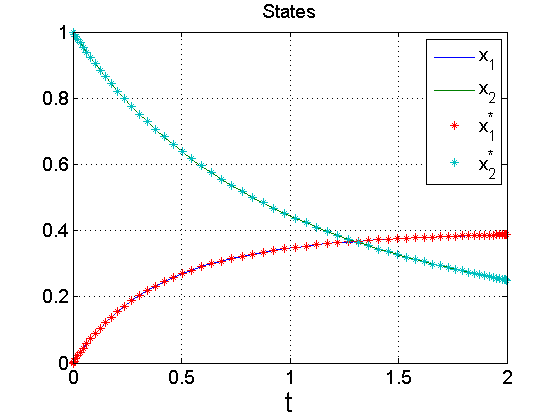
\includegraphics[width=1.\linewidth]{prob1States.png}
              \captionsetup{width=0.8\textwidth}
              \captionof{figure}{These are the states returned by Dido; the analytical solutions are plotted as as stars.  We see that the analytical solutions match the ones returned by Dido.  Also we see that Dido has satisfied the initial conditions specified in the problem statement.}
            \end{minipage}%
            \begin{minipage}{.5\textwidth}
              \centering
              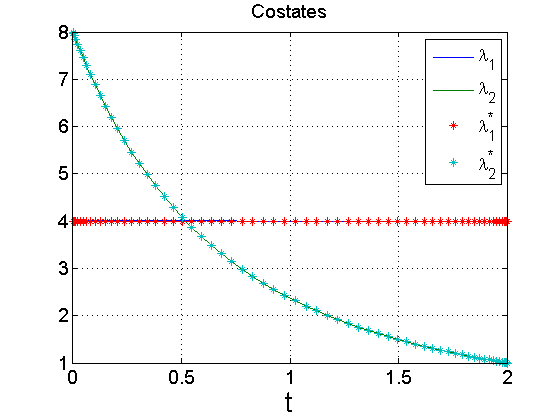
\includegraphics[width=1.\linewidth]{prob1Costates.png}
              \captionof{figure}{These are the costates returned by Dido, with the analytical solutions added to the graph.  We see that the Dido solution and the analytical solution match.  Also, the adjoint equations from Pontryagin's Necessary Condition states that the costate associated to $x_1$ is constant for all time, which is the case.  Similarly, the TTC gives that necessarily $\lambda_1=4$ for all time, and that $\lambda_2$ at the final time must be 1; both of which are satisfied on this plot  }
            \end{minipage}
         \end{figure}

       \begin{figure}[H]
            \centering
            \begin{minipage}{.5\textwidth}
              \centering
              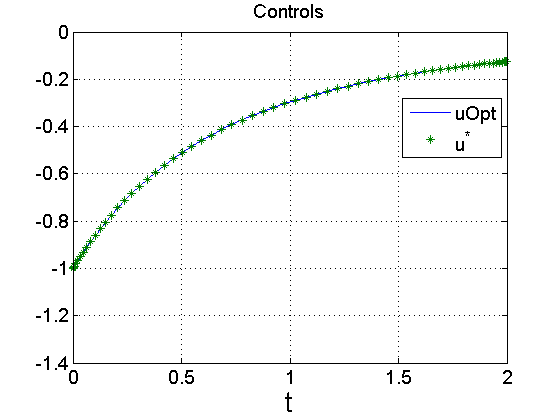
\includegraphics[width=1.\linewidth]{prob1Control.png}
              \captionsetup{width=0.8\textwidth}
              \captionof{figure}{This is the control returned by dido compared to the analytical solution given at the beginning of this section.  We see that the analytical solution matches with the control returned by Dido.}
            \end{minipage}%
            \begin{minipage}{.5\textwidth}
              \centering
              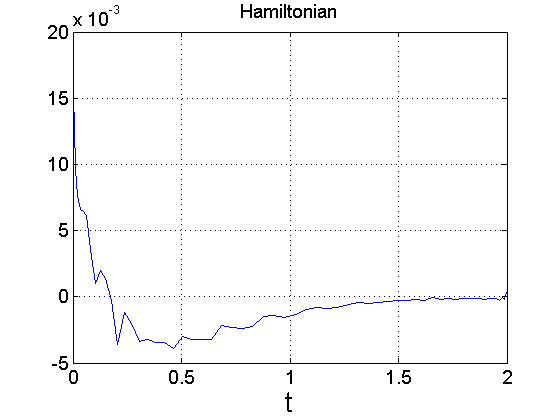
\includegraphics[width=1.\linewidth]{prob1Hamiltonian.png}
              \captionof{figure}{Pontryagin's Minimization Principal gives a necessary condition that the Hamiltonian must be constant for all time, and in this plot, we see that the Hamiltonian returned from Dido is nearly zero; we would say that this necessary condition has been met.}
            \end{minipage}
         \end{figure}

\item Define the state $x^T = \mat{x & y & \theta }\in\bbr^3$ with a control $u=\omega\in\bbr$, we consider the motion planing problem for Dubin's Vehicle:
    \begin{align*}
        P1 : \piece{ \text{Minimize} & J[x(\cdot), \omega(\cdot), t_f] = \int_{t_0}^{t_f}\omega^2(t)\,dt \\
                    \text{Subject to} & \dot x = \mat{\dot x \\ \dot y \\ \theta}
                                               = \mat{v\cos\theta \\ v\sin\theta \\ \omega}\triangleq f(x,\omega) \\
                     & t_0 = 0 \\
                     & x(t_0)=x^0\in\bbr^3 \\
                     & x(t_f)=x^f\in\bbr^3
                     }
    \end{align*}
    Where $v$ is a constant velocity and $x^0,x^f$ are given fixed values for the initial state and final state, and $t_f$ is free.
    \begin{enumerate}
      \item First we design a scaling to scale-out the constant velocity $v$.  Consider the following approach to scaling out $v$ from problem P1; consider $\hat t = \dfrac{t}{K_t}$ and $\hat\omega=\dfrac{\omega}{K_\omega}$ where $K_t$ and $K_\omega$ are constants to be determined (indeed, constants that will be chosen to scale-out $v$ from P1).  We must write all of the problem formulation in terms of hats:

          \textbf{Time}: We have that $\hat t_0= \dfrac{t_0}{K_t}=0$, and $\hat t_f=\dfrac{t_f}{K_t}$.  The end
          \textbf{Time}:  Endpoint Events.  Nothing changes here as the state variables are not scaled.  What does change, is just the time: $x(\hat t_0)=x^0$ and $x(\hat t_f)=x^f$
          \textbf{Dynamics}: Since no element of the state has been scaled, we need to only need to find $\libz{\cdot}{\hat t}$ for each of the state components: $x,y,\theta$.
          \begin{align} \label{eq:Scaled}
            \libz{x}{\hat t} &= \plibz{x}{ t}\plibz{t}{\hat t} = K_tv\cos\theta\\
            \libz{y}{\hat t} &= \plibz{y}{ t}\plibz{t}{\hat t} = K_tv\sin\theta\\
            \libz{\theta}{\hat t} &= \plibz{\theta}{ t}\plibz{t}{\hat t} = K_t\omega = K_tK_\omega\hat\omega
          \end{align}
          \textbf{Choosing $K_t,K_\omega$}: Since we want to remove the constant $v$ from the dynamics, by looking at \ref{eq:Scaled} we see that by choosing $K_t=\dfrac{1}{v}$ and $K_\omega=v$, we scale-out $v$ from the dynamics.
          \textbf{Cost Function}: $J$ must now be in terms of the scaled variables, so $J$ is a function of $x(\cdot), \hat\omega(\cdot)$ and $\hat t_f$.  Now $d\hat t = \frac{1}{K_t}\,dt$ and $\omega^2=k_\omega^2\hat\omega^2$ which gives us
          \begin{align*}
            \dint_{t_0}^{t_f} \omega^2(t)\,dt
                   &\longrightarrow \dint_{t_0/K_t}^{t_f/K_t}K_\omega^2\hat\omega^2(\hat t) K_t\,d\hat t\\
                   &= \dint_{\hat t_0}^{\hat t_f}\hat\omega^2(\hat t) \,d\hat t
          \end{align*}
          Where the scalars were dropped since minimization is invariant under scalar multiplication.  That is, minimizing $J$ is equivalent to minimizing $\alpha J$ where $\alpha>0$ is a scalar.

          Synthesizing the above, we have the the new formulation of P1 as
          \begin{align*}
            P1Scaled : \piece{ \text{Minimize} & J[x(\cdot), \hat\omega(\cdot), \hat t_f]
                                                     = \dint_{\hat t_0}^{\hat t_f}\hat\omega^2(\hat t) \,d\hat t \\
                    \text{Subject to} & \libz{x}{\hat t}= \mat{\libz{x}{\hat t} \\ \libz{x}{\hat t}\\ \libz{x}{\hat t}}
                                               = \mat{\cos\theta \\ \sin\theta \\ \hat\omega}\triangleq f(x,\omega) \\
                     & \hat t_0 = 0 \\
                     & x(\hat t_0)=x^0\in\bbr^3 \\
                     & x(\hat t_f)=x^f\in\bbr^3
                        }
          \end{align*}
      \item  We consider the following question: Given an optimal solution $S_1 = \cbrace{x(\cdot), \omega(\cdot), t_f}$ to P1 with $v=v_1$ (i.e.: a specific velocity).  Can we construct an optimal solution to P1 where the velocity constant is different, say $v=v_2$ ($v_1\neq v_2$)?  Yes, the answer is yes, and the work in part (a) of this problem hints at how this is true.  Given problem P1 with $v=v_1$, we can scale it to problem $P1Scaled$ with $\hat t = \dfrac{t}{K_t}$ and $\hat\omega=\dfrac{\omega}{K_\omega}$ where $K_t=\dfrac{1}{v_1}$ and $K_\omega=v_1$.  Solving $P1Scaled$, we receive the (scaled) state trajectory $S_s = \cbrace{x(\cdot), \omega(\cdot), t_f}$  Then, to recover the solution to $S_1$ we just have an un-scaling of $\omega = v_1\hat\omega$ and $t = \pdfrac{1}{v_1}\hat t$.  To get the solution when $v=v_2$, we need but change the un-scaling: $\omega = v_2\hat\omega$ and $t = \pdfrac{1}{v_2}\hat t$.   Attached to the appendix, is the scaled version of the Dubin's Vehicle with free end-time.
    \end{enumerate}


\item In the last problem, we consider the Brachistochrone problem where $e:\bbr\times\bbr\longrightarrow\bbr$ specifies the target set and $(x^0, y^0,v^0)\in\bbr^3$.  The state is $x=\mat{x\\y\\v}\in\bbr^3$ and the control $u=\theta\in\bbr$, and $g$ is acceleration due to gravity:
    \begin{align*}
            Brach: \piece{ \text{Minimize} & J[x(\cdot), u(\cdot), t_f] = t_f \\
                       \text{Subject to} & \dot x = \mat{\dot x \\ \dot y \\ \dot v} = \mat{ v\sin\theta \\ v\cos\theta \\ g\cos\theta}\triangleq f(x,u) \\
                       & t_0 = 0 \\
                       & x(t_0)=\mat{x^0\\y^0\\v^0} \\
                       & e(x(t_f))=0
                      }
    \end{align*}

    \begin{enumerate}
      \item Suppose that $\cbrace{x(\cdot), \theta(\cdot), t_f}$ is the optimal solution.  We will show that there exists $k\in\bbr$ such that
          \begin{align} \label{eq:Show}
            \mat{\dot x(t_f) \\ \dot y(t_f)}
                  = \mat{v(t_f)\sin\theta(t_f) \\ v(t_f)\cos\theta(t_f)}
                  = k\mat{\libzptrl{e}{x(t_f)} \\ \libzptrl{e}{y(t_f)}}
          \end{align}
          We denote the costates of the Brach problem as $\lambda^T=\mat{\lambda_x & \lambda_y & \lambda_v}$.  Since $H$ is time invariant, we have that $\libzptrl{H}{t}=0$, so $H[@t]$ is a constant for all time $t\in[t_0,t_f]$.  The HVC gives $H[@t_f]=-1$.  Therefore, we have that for all time $t\in[t_0,t_f]$, $H[@t]=-1$.  By the TTC, $\lambda_v(t_f)=0$, and combining this with the fact that $H[@t]=-1$ for all time, we have
          \begin{align} \label{eq:e1}
                \lambda_x(t_f)v(t_f)\sin\theta(t_f) + \lambda_y(t_f)v(t_f)\cos\theta(t_f) = -1
          \end{align}
          Combining  $\lambda_v(t_f)=0$, with the HMC (which gives $\libzptrl{H}{\theta}=0$), we have
          \begin{align} \label{eq:e2}
                \lambda_x(t_f)v(t_f)\cos\theta(t_f) + \lambda_y(t_f)v(t_f)\sin\theta(t_f) = 0
          \end{align}
          From \ref{eq:e1} and \ref{eq:e2}, we get
          \begin{align*}
            \lambda_x(t_f)v(t_f) &= -\sin\theta(t_f)\\
            \lambda_y(t_f)v(t_f) &= -\cos\theta(t_f)
          \end{align*}
          Now, we can write the TTC as $\lambda_x(t_f)=\nu\libzptrl{e}{x(t_f)}$, $\lambda_y(t_f)=\nu\libzptrl{e}{y(t_f)}$, where $\nu\in\bbr$ as our endpoint Lagrangian as $N_e=1$. Multiplying the above each by $-v(t_f)$ we have (where $k=-v(t_f)^2\nu$)
          \begin{align} \label{eq:L1}
            v(t_f)\sin\theta(t_f) = k\libzptrl{e}{x(t_f)}\\
            v(t_f)\cos\theta(t_f) = k\libzptrl{e}{y(t_f)}
          \end{align}
          And, since $\cbrace{x(\cdot), \theta(\cdot), t_f}$ is the optimal solution, the states satisfy the dynamics: That is, for all time $t\in[t_0,t_f]$ $\dot x = f(x,\theta)$.  Therefore
          \begin{align} \label{eq:L2}
            \mat{\dot x(t_f) \\ \dot y(t_f)}
                  = \mat{v(t_f)\sin\theta(t_f) \\ v(t_f)\cos\theta(t_f)}
          \end{align}
          And combining \ref{eq:L1} and \ref{eq:L2}, we have \ref{eq:Show}.
      \item The meaning of \ref{eq:Show} is that at the endpoint (i.e.: at the end time) the velocity vector (of the state) is parallel to the gradient of the target set at the end time.  Geometrically, this means that the curve of the brachistochrone strikes the target set orthogonally at the end time.  We demonstrate this by implementing the Brachistochrone problem in Dido with an initial condition $(x(t_0),y(t_0), v(t_0))=(0,0,0)$ and a target set of
          \begin{align*}
            e(x(t_f), y(t_f)) = (x(t_f)-5)^2 + (y(t_f)-1)^2 - 0.1^2
          \end{align*}
          which describes the target set as a circle.  The following plots were generated from the code given in the appendix.  All of the following figures were generated first by running 16 nodes with a guess (which is a straight line from the origin, the to center of the terminal circle), and then increasing the nodes, eventually up to 64 nodes, by using the guess as the previous run.

          \begin{figure}[H]
              \centering
              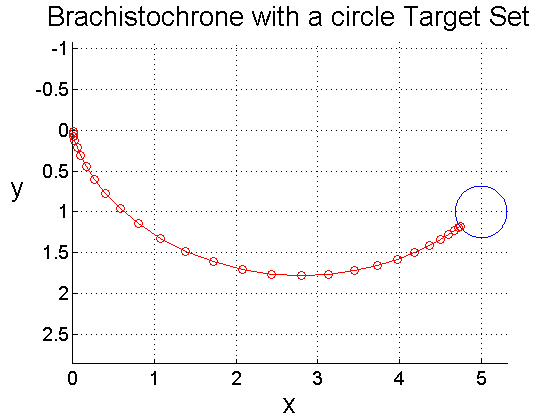
\includegraphics[width=.5\textwidth]{brachCurve.png}
              \captionsetup{width=0.8\textwidth}
              \captionof{figure}{ This is the curve returned by Dido that minimizes the transfer time of a particle starting at the origin at rest, and ending on the circle $(x-5)^2+(y-1)^2 -\pfrac{1}{\sqrt{10}}^2$.  From this plot, we can see that the curve strikes the terminal set in a perpendicular manner.  }
         \end{figure}


          \begin{figure}[H]
            \centering
            \begin{minipage}{.5\textwidth}
              \centering
              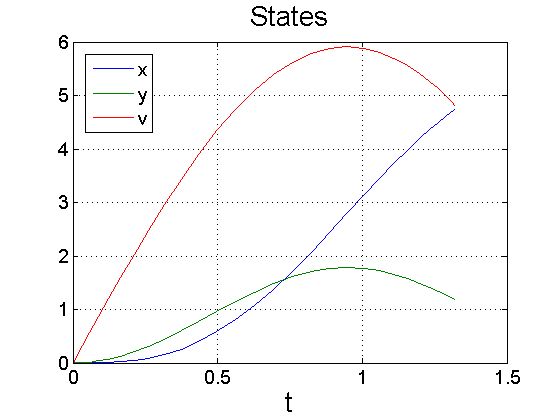
\includegraphics[width=1.\linewidth]{brachStates.png}
              \captionsetup{width=0.8\textwidth}
              \captionof{figure}{ The states to the Brachistochrone problem over time.  }
            \end{minipage}%
            \begin{minipage}{.5\textwidth}
              \centering
              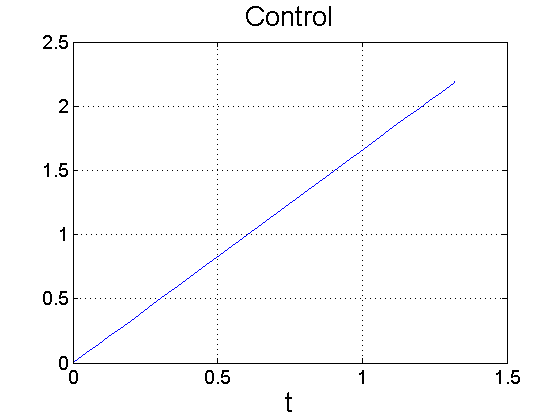
\includegraphics[width=1.\linewidth]{brachControl.png}
              \captionof{figure}{ The control $\theta$ returned by Dido, which is linear with respect to time $t$.  This matches the derivation in section 3.1 of Ross' text.}
            \end{minipage}
         \end{figure}

         \begin{figure}[H]
            \centering
            \begin{minipage}{.5\textwidth}
              \centering
              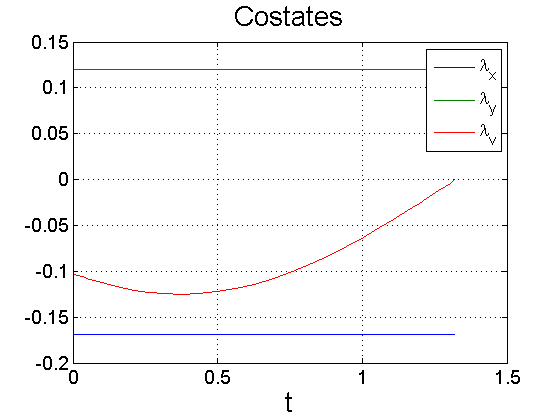
\includegraphics[width=1.\linewidth]{brachCostates.png}
              \captionsetup{width=0.8\textwidth}
              \captionof{figure}{ This plot are the costates returned by Dido.  Applying Pontryagin's Principal to the Brach problem, gives that extremal solutions necessarily have the costate associated to $x$ and $y$ to be constant for all time.  The TTC states that $\lambda_v(t_f)=0$: We see that the solution returned by Dido satisfies the necessary conditions associated to the costates.}
            \end{minipage}%
            \begin{minipage}{.5\textwidth}
              \centering
              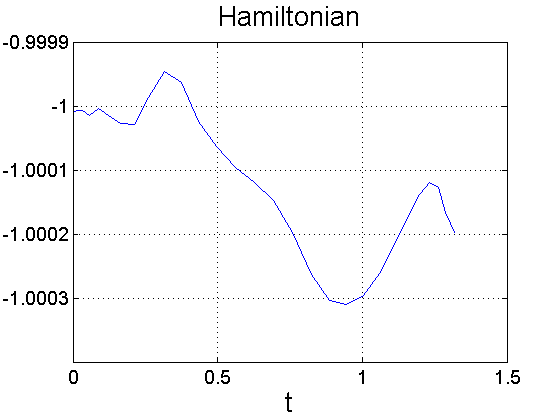
\includegraphics[width=1.\linewidth]{brachHamiltonian.png}
              \captionof{figure}{ This is the Hamiltonian returned by Dido.  Pontryagin's Principal give that, Necessarily the Hamiltonian must be -1 for all time $t\in[t_0,t_f]$, and we see in this figure that the result returned by Dido satisfies this Necessary condition.}
            \end{minipage}
         \end{figure}

    \end{enumerate}

\end{enumerate}


\newpage
\subsection*{Matlab Code}{
    To run each problem set, just make a sperate function-file for each function: costFun, dynamicsFun, eventFun, and one script file for the mainProblemFile.m
    \subsection*{Problem1}{
        \begingroup
        \fontsize{7pt}{7pt}
        \begin{verbatim}

function [ endPointCost, runningCost ] = costFun( primal )

    %Grab the final point of the states x1 and x2. i.e.: x1(tf) and x2(tf)
    x1f = primal.states(1, end);
    x2f = primal.states(2, end);

    u = primal.controls;

    endPointCost = 4*x1f + x2f;
    runningCost = 4*u.^2;

end

function [ XDot ] = dynamicsFun( primal )

    x2 = primal.states(2,:);
    u = primal.controls;

    x1Dot = x2.^3;
    x2Dot = u;

    %Dynamics go into XDot
    XDot = [ x1Dot; x2Dot ];

end

function [ endPointConstraints ] = eventFun( primal )

    %pull out the initial and final value of the state variable x
    x10 = primal.states(1,1);
    x20 = primal.states(2,1);

    endPointConstraints = [x10; x20];

end

%{
    Using Dido, we solve the optCtrl Problem 1 in HW #3
%}
clear all; close all;

%Analytical Extremal Solutions provided in the Homework
x1Star = @(t) 2/5 - 64./(5*(2+t).^5);
x2Star = @(t) 4./(2+t).^2;
uStar  = @(t) -8./(2+t).^3;
lambda1Star = @(t) 0*t+4;
lambda2Star = @(t) 64./(2+t).^3;

Nn = 32;
makeGuess = 0;
loadGuess = 1;


%Setting the box constraints to the states
x1L = -10; x2L = -10;
x1U =  10; x2U =  10;
bounds.lower.states = [x1L; x2L];
bounds.upper.states = [x1U; x2U];


%set the box constraints for the control
uL = -100; uU = 100;
bounds.lower.controls = [uL];
bounds.upper.controls = [uU];


%set the bounds for the initial and final time.  This problem is a fixed time problem.
t0 = 0;  tf = 2;
bounds.lower.time = [t0; tf];				
bounds.upper.time = [t0; tf];


%Endpoint constraint (i.e.: 'e' in the problem formulation).
x10 = 0;
x20 = 1;
bounds.lower.events = [x10; x20];
bounds.upper.events = bounds.lower.events;


%Pack the problem data into the problem structure 'optCtrlProb'
optCtrlProb.cost 	   = 'costFun';
optCtrlProb.dynamics   = 'dynamicsFun';
optCtrlProb.events     = 'eventFun';
optCtrlProb.bounds     = bounds;

%To use the previous run as an initial guess for the new run
if( loadGuess )
    load optCtrlPrimal primal;
    algorithm.guess = primal;
end

%A guesss to the problem: useful on a cold-run.  Our guess gives initial and final values
%for each state: x: 0 -> L, y:0->0, z:0->L
if( makeGuess )
    guess.states(1,:)	= [x10, x1U];
    guess.states(2,:)	= [x20, x2U];

    guess.controls(1,:)		= [0, 0];

    guess.time			    = [t0, tf];

    algorithm.guess = guess;
end

%Here is how to run DIDO in accurate mode.
% algorithm.mode = 'accurate';

%The number of nodes Nn is Nn+1 sample points taken inbetween the initial and
%final time bounds.  Increase Nn for greater accuracy.  Hence Nn+1 points on the
%interval [0,1]
algorithm.nodes = [Nn];

% call dido and record the execution time
tStart= cputime;
    [cost, primal, dual] = dido(optCtrlProb, algorithm);
runTime = cputime-tStart;

%%%%%%%%%%%%%%%%%%-----Pretty Plot Code Follows-----%%%%%%%%%%%%%%%%%%

disp(strcat('Dido executed in:', ' ' ,num2str(runTime), ' seconds.'));
disp(strcat('Minimized Cost:', ' ' ,num2str(cost), ' cost units.'));

%Unpack the optimal solution from DIDO's primal structure
xOpt = primal.states;
uOpt = primal.controls;
tNodes = primal.nodes;
costates = dual.dynamics;


%%%Pretty Plot Code%%%

figure;
    plot(tNodes, xOpt, ...
         tNodes, x1Star(tNodes), '*', ...
         tNodes, x2Star(tNodes), '*');
    title('States');
    xlabel('t', 'FontSize', 20);
    legend('x_1', 'x_2', 'x_1^*', 'x_2^*');
    grid on;

figure
    plot(tNodes, uOpt, ...
         tNodes, uStar(tNodes), '*');
    title('Controls');
    xlabel('t', 'FontSize', 20);
    legend('uOpt', 'u^*');
    grid on;

figure;
    plot(tNodes, dual.Hamiltonian);
    title('Hamiltonian');
    xlabel('t', 'FontSize', 20);
    grid on;


figure;
    plot(tNodes, costates, ...
         tNodes, lambda1Star(tNodes), '*', ...
         tNodes, lambda2Star(tNodes), '*' );
    title('Costates')
    xlabel('t', 'FontSize', 20);
    legend('\lambda_1', '\lambda_2', '\lambda_1^*', '\lambda_2^*');
    grid on;


save optCtrlPrimal;

%
% end mainProblemFile.m
%
        \end{verbatim}
        \endgroup
    }

    \subsection*{Problem2}{
        \begingroup
        \fontsize{7pt}{7pt}
        \begin{verbatim}
function [ endPointCost, runningCost ] = costFun( primal )

    omegaHat = primal.controls(1,:);

    endPointCost = 0;
    runningCost = omegaHat.^2;

end


function [ XDot ] = dynamicsFun( primal )

    theta = primal.states(3,:);
    omegaHat = primal.controls;

    xDot = cos(theta);
    yDot = sin(theta);
    thetaDot = omegaHat;

    %Dynamics go into XDot
    XDot = [ xDot; yDot; thetaDot ];
end


function [ endPointConstraints ] = eventFun( primal )

    %pull out the initial and final value of the state variable x
    initialStates = primal.states(:,1);
    finalStates = primal.states(:,end);

    %The order of the endpoint constraints is [x0;v0;xf;vf], this has been set in the main
    %file.
    endPointConstraints = [initialStates; finalStates];


end


%{
    Here we look at a Dubins Vehicle: We control the turning rate and minimize the L2 norm
    of the turning rate (smooth ride)
    State: x y theta
    Control: omega (turning rate)
    Dynamics:
         xDot = v*cos(theta)
         yDot = v*sin(theta)
         thetaDot = omega
    So, we have a 3dim state and the control is one dim.

    We are given the initial position and orientation of the car, and we are given the
    final position and and orientation.  We are also given the start and end times.  Given
    this information we look for a curve that satisfies the endpoint constraints (initial
    and final) while minimizing the rate of change of the car turning.
%}
clear all; close all;

global Kt Komega;

v=0.01;

Kt = 1/v;
Komega = v;

Nn = 16;
makeGuess = 1;
loadGuess = 0;
runInAccurateMode = 0;

%Setting the box constraints to the OptCtrl problem.
xL=-10;  yL=-10;  thetaL=-2*pi;
xU=10;   yU=10;   thetaU=2*pi;
bounds.lower.states = [xL;yL;thetaL];
bounds.upper.states = [xU;yU;thetaU];


%Set the box constraints for the control u.
omegaLHat = -100/Komega;
omegaUHat = 100/Komega;
bounds.lower.controls = [omegaLHat];
bounds.upper.controls = [omegaUHat];


%set the bounds for the initial and final time.
t0Hat = 0/Kt;  tfHat = 300/Kt;
bounds.lower.time = [t0Hat; t0Hat];				
bounds.upper.time = [t0Hat; tfHat];


%Endpoint constraint (i.e.: 'e' in the problem formulation).  We start and end at a
%specific point and orientation
x0 = 0; y0 = 0;
xf = 1; yf = 1;
theta0 = pi/4;
thetaf = pi/4;
bounds.lower.events = [x0; y0; theta0; xf; yf; thetaf];
bounds.upper.events = bounds.lower.events;


dubinsVeh.cost 	   = 'costFun';
dubinsVeh.dynamics = 'dynamicsFun';
dubinsVeh.events   = 'eventFun';
dubinsVeh.bounds   = bounds;

%To use the previous run as an initial guess for the new run
if( loadGuess )
    load optCtrlPrimal primal;
    algorithm.guess = primal;
end

%A guesss to the problem: useful on a cold-run.  Our guess gives initial and final values
%for each state: x: 0 -> L, y:0->0, z:0->L
if( makeGuess )
    guess.states(1,:)	= [x0, xf];
    guess.states(2,:)	= [y0, yf];
    guess.states(3,:)	= [theta0, thetaf];

    guess.controls(1,:)		= [0, 0];

    guess.time			    = [t0Hat, .5*tfHat];

    algorithm.guess = guess;
end

if( runInAccurateMode )
    algorithm.mode = 'accurate';
end

%The number of nodes Nn is Nn+1 sample points taken inbetween the initial and
%final time bounds.  Increase Nn for greater accuracy.  Hence Nn+1 points on the
%interval [0,1]
algorithm.nodes = [Nn];

% call dido and record the execution time
tStart= cputime;
    [cost, primal, dual] = dido(dubinsVeh, algorithm);
runTime = cputime-tStart;

%%%%%%%%%%%%%%%%%%-----Pretty Plot Code Follows-----%%%%%%%%%%%%%%%%%%

disp(strcat('Dido executed in:', ' ' ,num2str(runTime), ' seconds.'));
disp(strcat('Cost Minimized:', ' ' ,num2str(cost), ' (cost units).'));

%Unpack the optimal solution from DIDO's primal structure
xOpt = primal.states;
omegaOpt = Komega*primal.controls;
tNodes = Kt*primal.nodes;

figure;
    plot(xOpt(1,:), xOpt(2,:));
    title( 'Curve Minimizing Engergy', 'FontSize', 20 );
    xlabel('x', 'FontSize', 20);
    ylabel('y', 'FontSize', 20);
    axis equal;

figure;
    plot(tNodes, xOpt);
    title('States', 'FontSize', 20);
    legend('x', 'y', '\theta');
    xlabel('t');

figure;
    plot(tNodes, omegaOpt)
    title('Unscaled Control', 'FontSize', 20);
    xlabel('t');
    ylabel('u');

figure;
    plot(primal.nodes, primal.controls)
    title('Scaled Control', 'FontSize', 20);
    xlabel('t');
    ylabel('u');

%Plot the Control Hamiltonian.
figure;
plot(tNodes, dual.Hamiltonian);
    title('Hamiltonian', 'FontSize', 20);
    legend('H');
    xlabel('time', 'FontSize', 20);
    ylabel('Hamiltonian Value', 'FontSize', 20);


%Plot the costates
figure;
plot(tNodes, Kt*dual.dynamics);
    title('Costates', 'FontSize', 20)
    xlabel('time', 'FontSize', 20);
    ylabel('costates', 'FontSize', 20);
    legend('\lambda_x', '\lambda_y', '\lambda_\theta');

save optCtrlPrimal;

%
% end mainProblemFile.m
%
        \end{verbatim}
        \endgroup
    }

    \subsection*{Problem3}{
        \begingroup
        \fontsize{7pt}{7pt}
        \begin{verbatim}
function [ endPointCost, runningCost ] = costFun( primal )

    tf = primal.nodes(end);

    endPointCost = tf;
    runningCost = 0;

end


function [ XDot ] = dynamicsFun( primal )

    global g;

    v = primal.states(3,:);
    theta = primal.controls;

    xDot = v.*sin(theta);
    yDot = v.*cos(theta);
    vDot = g*cos(theta);

    %Dynamics go into XDot
    XDot = [xDot; yDot; vDot ];
end


function [ endPointConstraints ] = eventFun( primal )

    global e;

    %pull out the initial and final value of the state variable x
    x0 = primal.states(1,1);
    xf = primal.states(1,end);
    y0 = primal.states(2,1);
    yf = primal.states(2,end);
    v0 = primal.states(3,1);


    %The order of the endpoint constraints, this has been set in the main file.
    endPointConstraints = zeros(4,1);

    endPointConstraints(1) = x0;
    endPointConstraints(2) = y0;
    endPointConstraints(3) = v0;
    endPointConstraints(4) = e(xf,yf);

end


%{
    Using Dido, we solve the brachistochrone problem where we must end on a circle.
%}
clear all; close all;

%{
    g: Gravit Constant , Units m/s^2
    e: Function representing the circle the particle must land upon at the final time.
%}
global g e;


g = 9.8;
h = 5; k = 1; r =1/sqrt(10);
e = @(xf, yf) (xf-h)^2 + (yf-k)^2 - r^2;


Nn = 32;
makeGuess = 0;
loadGuess = 1;

%Setting the box constraints to the states
xL = 0; xU = 20;
yL = 0; yU = 20;
vL = 0; vU = 20;
bounds.lower.states = [xL; yL; vL];
bounds.upper.states = [xU; yU; vU];


%set the box constraints for the control
thetaL = 0; thetaU = pi;
bounds.lower.controls = [thetaL];
bounds.upper.controls = [thetaU];


%set the bounds for the initial and final time.  The final time is free, and the initial
%time is fixed
t0 = 0;  tfMax = 10;
bounds.lower.time = [t0; t0];				
bounds.upper.time = [t0; tfMax];


%Endpoint constraints: We are given an initial condition, and must end on a circle.  The
%last constraint defines e(x(tf),y(tf))=0
x0 = 0; y0=0; v0=0;
bounds.lower.events = [x0; y0; v0; 0];
bounds.upper.events = bounds.lower.events;


%Pack the problem data into the problem structure 'optCtrlProb'
optCtrlProb.cost 	   = 'costFun';
optCtrlProb.dynamics   = 'dynamicsFun';
optCtrlProb.events     = 'eventFun';		
optCtrlProb.bounds     = bounds;

%To use the previous run as an initial guess for the new run
if( loadGuess )
    load optCtrlPrimal primal;
    algorithm.guess = primal;
end

%A guesss to the problem: useful on a cold-run.  Our guess is a straight line to the
%center of the circle we must land upon.
if( makeGuess )
    guess.states(1,:)	= [x0, h];
    guess.states(2,:)	= [y0, k];
    guess.states(3,:)	= [v0, vU];

    guess.controls(1,:)		= [0, 0];

    guess.time			    = [t0, tfMax];

    algorithm.guess = guess;
end

%Here is how to run DIDO in accurate mode.
% algorithm.mode = 'accurate';

%The number of nodes Nn is Nn+1 sample points taken inbetween the initial and
%final time bounds.  Increase Nn for greater accuracy.  Hence Nn+1 points on the
%interval [0,1]
algorithm.nodes = [Nn];

% call dido and record the execution time
tStart= cputime;
    [cost, primal, dual] = dido(optCtrlProb, algorithm);
runTime = cputime-tStart;

%%%%%%%%%%%%%%%%%%-----Pretty Plot Code Follows-----%%%%%%%%%%%%%%%%%%

disp(strcat('Dido executed in:', ' ' ,num2str(runTime), ' seconds.'));
disp(strcat('Minimized Cost:', ' ' ,num2str(cost), ' cost units.'));

%Unpack the optimal solution from DIDO's primal structure
xOpt = primal.states;
uOpt = primal.controls;
tNodes = primal.nodes;


%%% Pretty Plot Code %%%

%Plot the Brach curve, as well as the terminal circle
figure;
hold on;
    tDom = 0:0.01:2*pi;
    plot(h+r*cos(tDom), k+r*sin(tDom));
    plot(xOpt(1,:),xOpt(2,:),'ro-');
    title('Brachistochrone with a circle Target Set','fontSize',20);
    xlabel('x','fontSize',20);
    ylabel('y   ','fontSize',20, 'Rotation', 0);
    set(gca,'YDir','reverse');
    grid on;
    axis equal;
hold off;

figure;
    plot(tNodes, xOpt);
    title('States', 'fontSize',20);
    xlabel('t','fontSize',20);
    grid on;
    legend('x','y','v');

figure
    plot(tNodes, uOpt);
    title('Control', 'fontSize',20);
    grid on;
    xlabel('t','fontSize',20);

figure;
    plot(tNodes, dual.Hamiltonian);
    title('Hamiltonian', 'fontSize',20);
    grid on;
    xlabel('t','fontSize',20);

figure;
    plot(tNodes, dual.dynamics);
    title('Costates', 'fontSize',20);
    xlabel('t','fontSize',20);
    grid on;
    legend('\lambda_x', '\lambda_y', '\lambda_v');

save optCtrlPrimal;

%
% end mainProblemFile.m
%

        \end{verbatim}
        \endgroup
    }
}

\end{document} 